\section{Analysis: Task predictability with the ladder}
%\label{sec:analyses}
\label{sec_variance_analysis}

% \akshita{should add c4 and taskCE var analysis here; c4 will be just a single number. adding taskCE to table is trickier, so as before, we can say we show bpb as example. it will be good to have taskCE SD numbers in appendix though.}

Some tasks are inherently more challenging to predict reliably with the ladder models; 
for example, a test set with an inadequate sample size, low-quality test instances or questions that are too difficult for small models. We anticipate three sources of prediction failure: 
%(1) high variance in task loss, (2) high variance in task accuracy; higher spread of prediction targets, (3) random-chance task accuracy in smaller ladder models due to task difficulty.

\begin{itemize}[leftmargin=16pt]
\item High variance in intermediate loss; less reliable data points for function fitting.
\item High variance in task accuracy; higher spread of prediction targets.
\item Random-chance task accuracy in smaller ladder models due to task difficulty.
\end{itemize}

We try to determine which tasks will exhibit high prediction errors, using task loss as the intermediate feature. We use the intermediate checkpoints of the largest ladder model (1B-1xC) to measure the noise for task loss and task accuracy. Failure due to random-chance accuracy is discussed when predicting multiple-choice tasks in \S\ref{sec:mc}.

\tightparagraph{Variance analysis.}

We compute the standard deviation of the last $n$ training checkpoints of 1B-10xC ($\text{SD}_n$). We also compute relative SD (also called the coefficient of variation) to compare between tasks:

\begin{equation} \label{eq:cv}
\text{Relative SD}_{n} = \frac{\text{SD (final $n$ checkpoints)}}{\text{Mean (final $n$ checkpoints)}} \times 100\%
\end{equation}

A task where ladder models exhibit a higher standard deviation across adjacent evaluated checkpoints potentially indicates a higher prediction error for the target models. To illustrate $\text{SD}_n$, we show the intermediate checkpoints for the largest ladder model on OpenBookQA and MMLU in \autoref{fig:variance_small}, where we find that $\text{SD}_{10}$ captures the apparent noise between adjacent training checkpoints. 

\begin{figure}[t]
\centering
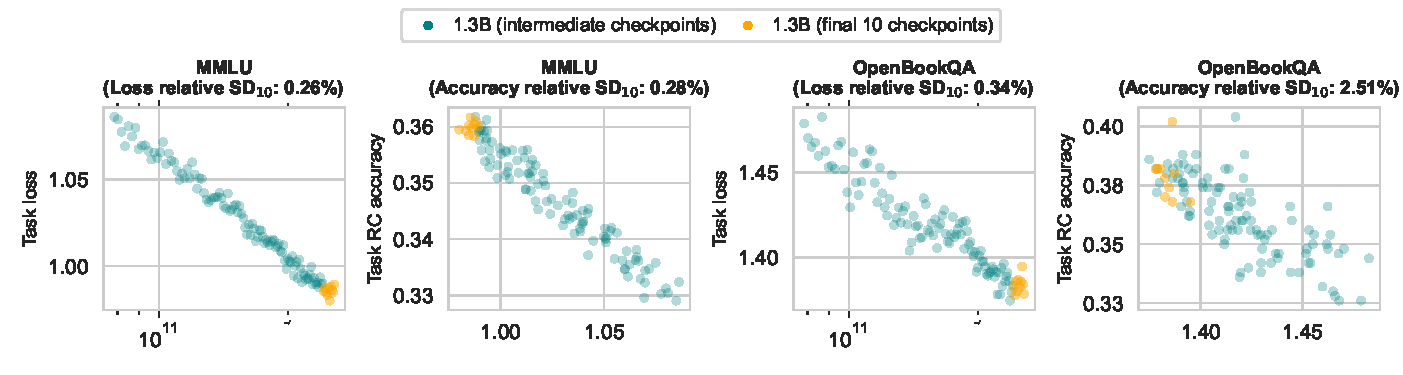
\includegraphics[scale=0.6]{images/variance_analysis/variance_one_row.pdf}
\vspace{-12pt}
\caption{
Relative SD over the final 10 checkpoints (SD$_{10}$) for the 1B-10xC ladder model on MMLU and OpenBookQA. 
OBQA metrics appear noisier than MMLU, resulting in a higher SD$_{10}$.
Tasks with high intermediate checkpoint noise indicate higher prediction error (\autoref{tab:variance_analysis}). 
Results across all tasks are in \autoref{fig:variance}. 
}
\label{fig:variance_small}
\vspace{-8pt}
\end{figure}

% \begin{table*}[!h]
% \small
% % \setlength{\tabcolsep}{3pt}
% \centering
% \begin{tabular}{l | c c c}
% \toprule
% Task & Loss CV & Accuracy CV \\
% \midrule
% mmlu avg var & 0.3\% & 0.5\% \\
% hellaswag 5-shot & 0.2\% & 1.0\% \\
% arc easy 5-shot & \cellcolor{red!30}1.0\% & 1.0\% \\
% arc challenge 5-shot & 0.4\% & \cellcolor{red!30}3.1\% \\
% boolq 5-shot & \cellcolor{red!30}2.7\% & \cellcolor{red!30}8.1\% \\
% csqa 5-shot & 0.6\% & 0.9\% \\
% openbookqa 5-shot & 0.4\% & 1.8\% \\
% piqa 5-shot & 0.3\% & 0.6\% \\
% socialiqa 5-shot & 0.5\% & 1.4\% \\
% winogrande 5-shot & \cellcolor{red!30}0.8\% & 0.8\% \\
% \midrule
% Average & 0.7\% & 1.9\% \\
% \bottomrule
% \end{tabular}
% \caption{
%     Coefficient of variation ($CV_{20}$) for the loss and accuracy of each task, as based on the trained 1B-10xC model curves. The numbers highlighted in red correspond to the tasks with higher than average CV  in each column.
% }
% \label{tab:variance_analysis}
% % \vspace{-16pt}
% \end{table*}

\begin{table*}[t]
\small
% \setlength{\tabcolsep}{3pt}
\centering
\caption{
Absolute and relative standard deviation of last 10 training checkpoints (SD$_{10}$) for the 1B-10xC model on task loss and accuracy, and relative error for predicting the 7B-4T model on task loss (step 1 only), accuracy (step 2 only) and chained accuracy (step 1 and step 2). 
We observe that tasks with above-average SD$_{10}$ for 1B-10xC, highlighted in \textcolor{red!80}{red}, tend to have high prediction errors for the 7B-4T model. 
In particular, we observe a strong Pearson correlation between loss SD$_{10}$ and accuracy prediction error ($r=0.821, p=0.004$).
}

% \begin{tabular}{l | c c c c c}
% \toprule
% Task & SD (Loss) & Relative SD (Loss) & SD (Accuracy) & Relative SD (Accuracy) \\
% \midrule
% mmlu avg var & 0.3\% & 0.3\% & 0.2\% & 0.5\% \\
% hellaswag 5-shot & 0.1\% & 0.2\% & 0.7\% & 1.0\% \\
% arc easy 5-shot & \cellcolor{red!30}0.7\% & 1.0\% & 0.7\% & 1.0\% \\
% arc challenge 5-shot & 0.3\% & 0.4\% & \cellcolor{red!30}1.2\% & 3.1\% \\
% boolq 5-shot & \cellcolor{red!30}1.1\% & 2.7\% & \cellcolor{red!30}4.6\% & 8.1\% \\
% csqa 5-shot & 0.6\% & 0.6\% & 0.6\% & 0.9\% \\
% openbookqa 5-shot & \cellcolor{red!30}0.6\% & 0.4\% & 0.7\% & 1.8\% \\
% piqa 5-shot & 0.3\% & 0.3\% & 0.5\% & 0.6\% \\
% socialiqa 5-shot & 0.5\% & 0.5\% & 0.7\% & 1.4\% \\
% winogrande 5-shot & \cellcolor{red!30}1.2\% & 0.8\% & 0.5\% & 0.8\% \\
% \midrule
% Average & 0.6\% & 0.7\% & 1.0\% & 1.9\% \\
% \bottomrule
% \end{tabular}

% \begin{tabular}{l | c c c c | c c c}
% \toprule
%  & \multicolumn{4}{c}{\textbf{Variance Analysis on 1B}} & \multicolumn{3}{c}{\textbf{Predictions for 7B}} \\
%  & \makecell{Loss \\ SD} & \makecell{Loss \\ CV} & \makecell{Accuracy \\ SD} & \makecell{Accuracy \\ CV} & \makecell{Loss \\ Rel Error} & \makecell{Accuracy \\Rel Error} & \makecell{Stacked \\ Rel Error} \\
% Task &  &  &  &  &  &  &  \\
% \midrule
% winogrande 5-shot & \cellcolor{red!30}1.17 \% & 0.77 \% & 0.49 \% & 0.79 \% & 0.74 \% & 25.10 \% & 26.27 \% \\
% boolq 5-shot & \cellcolor{red!30}1.06 \% & 2.68 \% & \cellcolor{red!30}4.56 \% & 8.12 \% & 45.20 \% & 20.58 \% & 25.80 \% \\
% arc-e 5-shot & \cellcolor{red!30}0.65 \% & 0.96 \% & 0.71 \% & 0.98 \% & 20.11 \% & 9.66 \% & 15.83 \% \\
% openbookqa 5-shot & \cellcolor{red!30}0.59 \% & 0.43 \% & 0.68 \% & 1.84 \% & 4.34 \% & 11.31 \% & 18.77 \% \\
% csqa 5-shot & 0.56 \% & 0.55 \% & 0.57 \% & 0.89 \% & 5.75 \% & 0.94 \% & 1.55 \% \\
% socialiqa 5-shot & 0.53 \% & 0.49 \% & 0.72 \% & 1.38 \% & 6.34 \% & 2.85 \% & 6.22 \% \\
% arc-c 5shot & 0.34 \% & 0.41 \% & \cellcolor{red!30}1.23 \% & 3.12 \% & 3.23 \% & 6.41 \% & 0.49 \% \\
% mmlu avg var & 0.32 \% & 0.29 \% & 0.18 \% & 0.52 \% & 2.20 \% & 0.69 \% & 3.69 \% \\
% piqa 5-shot & 0.30 \% & 0.29 \% & 0.47 \% & 0.63 \% & 0.34 \% & 1.06 \% & 0.84 \% \\
% hellaswag 5-shot & 0.13 \% & 0.17 \% & 0.66 \% & 1.03 \% & 2.13 \% & 0.99 \% & 1.82 \% \\
% \bottomrule
% \end{tabular}


\begin{tabular}{l | C{33pt} C{33pt} C{33pt} C{33pt} | C{33pt} C{33pt} C{33pt}}
% \begin{tabular}{l | c c c c | c c c}
\toprule
 & \multicolumn{4}{c}{\textbf{Std. dev. of final 1B checkpoints}} & \multicolumn{3}{c}{\textbf{Predictions for 7B-4T}} \\
Task 
& \makecell{Loss \\ SD$_{10}$} 
& \makecell{Loss \\ \% SD$_{10}$} 
% & \makecell{Accuracy\\SD$_{10}$} 
& {\hspace{-0.2cm}\makecell{Accuracy\\SD$_{10}$}}
& {\hspace{-0.2cm}\makecell{Accuracy\\\% SD$_{10}$}} 
& \makecell{Loss \\ \% Error} 
& {\hspace{-0.2cm}\makecell{Accuracy\\\% Error}} 
& {\hspace{-0.1cm}\makecell{Chained\\\% Error}} \\
\midrule
% WinoGrande & \cellcolor{red!30}1.15 \% & \cellcolor{red!30}0.75 \% & 0.48 \% & 0.77 \% & 4.52 \% & \cellcolor{red!30}23.67 \% & \cellcolor{red!30}8.86 \% \\
% BoolQ & \cellcolor{red!30}0.68 \% & \cellcolor{red!30}1.76 \% & \cellcolor{red!30}1.86 \% & \cellcolor{red!30}2.86 \% & \cellcolor{red!30}11.38 \% & 4.29 \% & 1.82 \% \\
% CommonsenseQA & \cellcolor{red!30}0.56 \% & \cellcolor{red!30}0.56 \% & 0.35 \% & 0.55 \% & \cellcolor{red!30}11.72 \% & 1.00 \% & 4.22 \% \\
% OpenBoolQA & \cellcolor{red!30}0.47 \% & 0.34 \% & \cellcolor{red!30}0.95 \% & \cellcolor{red!30}2.51 \% & 1.30 \% & \cellcolor{red!30}8.19 \% & \cellcolor{red!30}10.59 \% \\
% ARC-Easy & \cellcolor{red!30}0.45 \% & \cellcolor{red!30}0.66 \% & 0.43 \% & 0.61 \% & \cellcolor{red!30}13.28 \% & 4.49 \% & \cellcolor{red!30}9.42 \% \\
% ARC-Challenge & 0.37 \% & 0.40 \% & 0.40 \% & \cellcolor{red!30}1.00 \% & \cellcolor{red!30}6.96 \% & \cellcolor{red!30}7.59 \% & \cellcolor{red!30}16.87 \% \\
% MMLU & 0.26 \% & 0.26 \% & 0.10 \% & 0.28 \% & 1.28 \% & 0.27 \% & 1.28 \% \\
% Social IQa & 0.24 \% & 0.23 \% & 0.32 \% & 0.61 \% & 4.32 \% & 4.73 \% & 1.98 \% \\
% PIQA & 0.19 \% & 0.19 \% & 0.24 \% & 0.31 \% & 2.04 \% & 2.28 \% & 1.01 \% \\
% HellaSwag & 0.07 \% & 0.09 \% & 0.16 \% & 0.25 \% & 0.29 \% & 1.05 \% & 1.44 \% \\

Winogrande & \cellcolor{red!30}0.0115 & \cellcolor{red!30}0.75 \% & 0.0048 & 0.77 \% & 4.5 \% & \cellcolor{red!30}23.7 \% & \cellcolor{red!30}8.9 \% \\
BoolQ & \cellcolor{red!30}0.0068 & \cellcolor{red!30}1.76 \% & \cellcolor{red!30}0.0186 & \cellcolor{red!30}2.86 \% & \cellcolor{red!30}11.4 \% & 4.3 \% & 1.8 \% \\
CommonsenseQA & \cellcolor{red!30}0.0056 & \cellcolor{red!30}0.56 \% & 0.0035 & 0.55 \% & \cellcolor{red!30}11.7 \% & 1.0 \% & 4.2 \% \\
OpenBookQA & \cellcolor{red!30}0.0047 & 0.34 \% & \cellcolor{red!30}0.0095 & \cellcolor{red!30}2.51 \% & 1.3 \% & \cellcolor{red!30}8.2 \% & \cellcolor{red!30}10.6 \% \\
ARC-Easy & \cellcolor{red!30}0.0045 & \cellcolor{red!30}0.66 \% & 0.0043 & 0.61 \% & \cellcolor{red!30}13.3 \% & 4.5 \% & \cellcolor{red!30}9.4 \% \\
ARC-Challenge & 0.0037 & 0.40 \% & 0.0040 & \cellcolor{red!30}1.00 \% & \cellcolor{red!30}7.0 \% & \cellcolor{red!30}7.6 \% & \cellcolor{red!30}16.9 \% \\
MMLU & 0.0026 & 0.26 \% & 0.0010 & 0.28 \% & 1.3 \% & 0.3 \% & 1.3 \% \\
Social IQa & 0.0024 & 0.23 \% & 0.0032 & 0.61 \% & 4.3 \% & 4.7 \% & 2.0 \% \\
PIQA & 0.0019 & 0.19 \% & 0.0024 & 0.31 \% & 2.0 \% & 2.3 \% & 1.0 \% \\
HellaSwag & 0.0007 & 0.09 \% & 0.0016 & 0.25 \% & 0.3 \% & 1.1 \% & 1.4 \% \\
\bottomrule
\end{tabular}

\label{tab:variance_analysis}
\vspace{-12pt}
\end{table*}



We present $\text{SD}_{10}$ for the 1B-10xC model \autoref{tab:variance_analysis}, alongside prediction errors for the 7B-4T model.
Benchmarks with low SD$_{10}$ (e.g. MMLU and HellaSwag), also have low prediction errors for the target, indicating these tasks are easier for the ladder to predict.
We also find that Loss SD$_{10}$ is correlated with step 2 accuracy error (Pearson $r=0.821, p=0.004$ for 7B-4T and $r=0.855, p=0.002$ for 13B-5T).
Thus, SD$_{10}$ can be reported alongside predictions to explain which benchmarks may have high error before running the target model.

% \begin{figure*}[t]
\centering
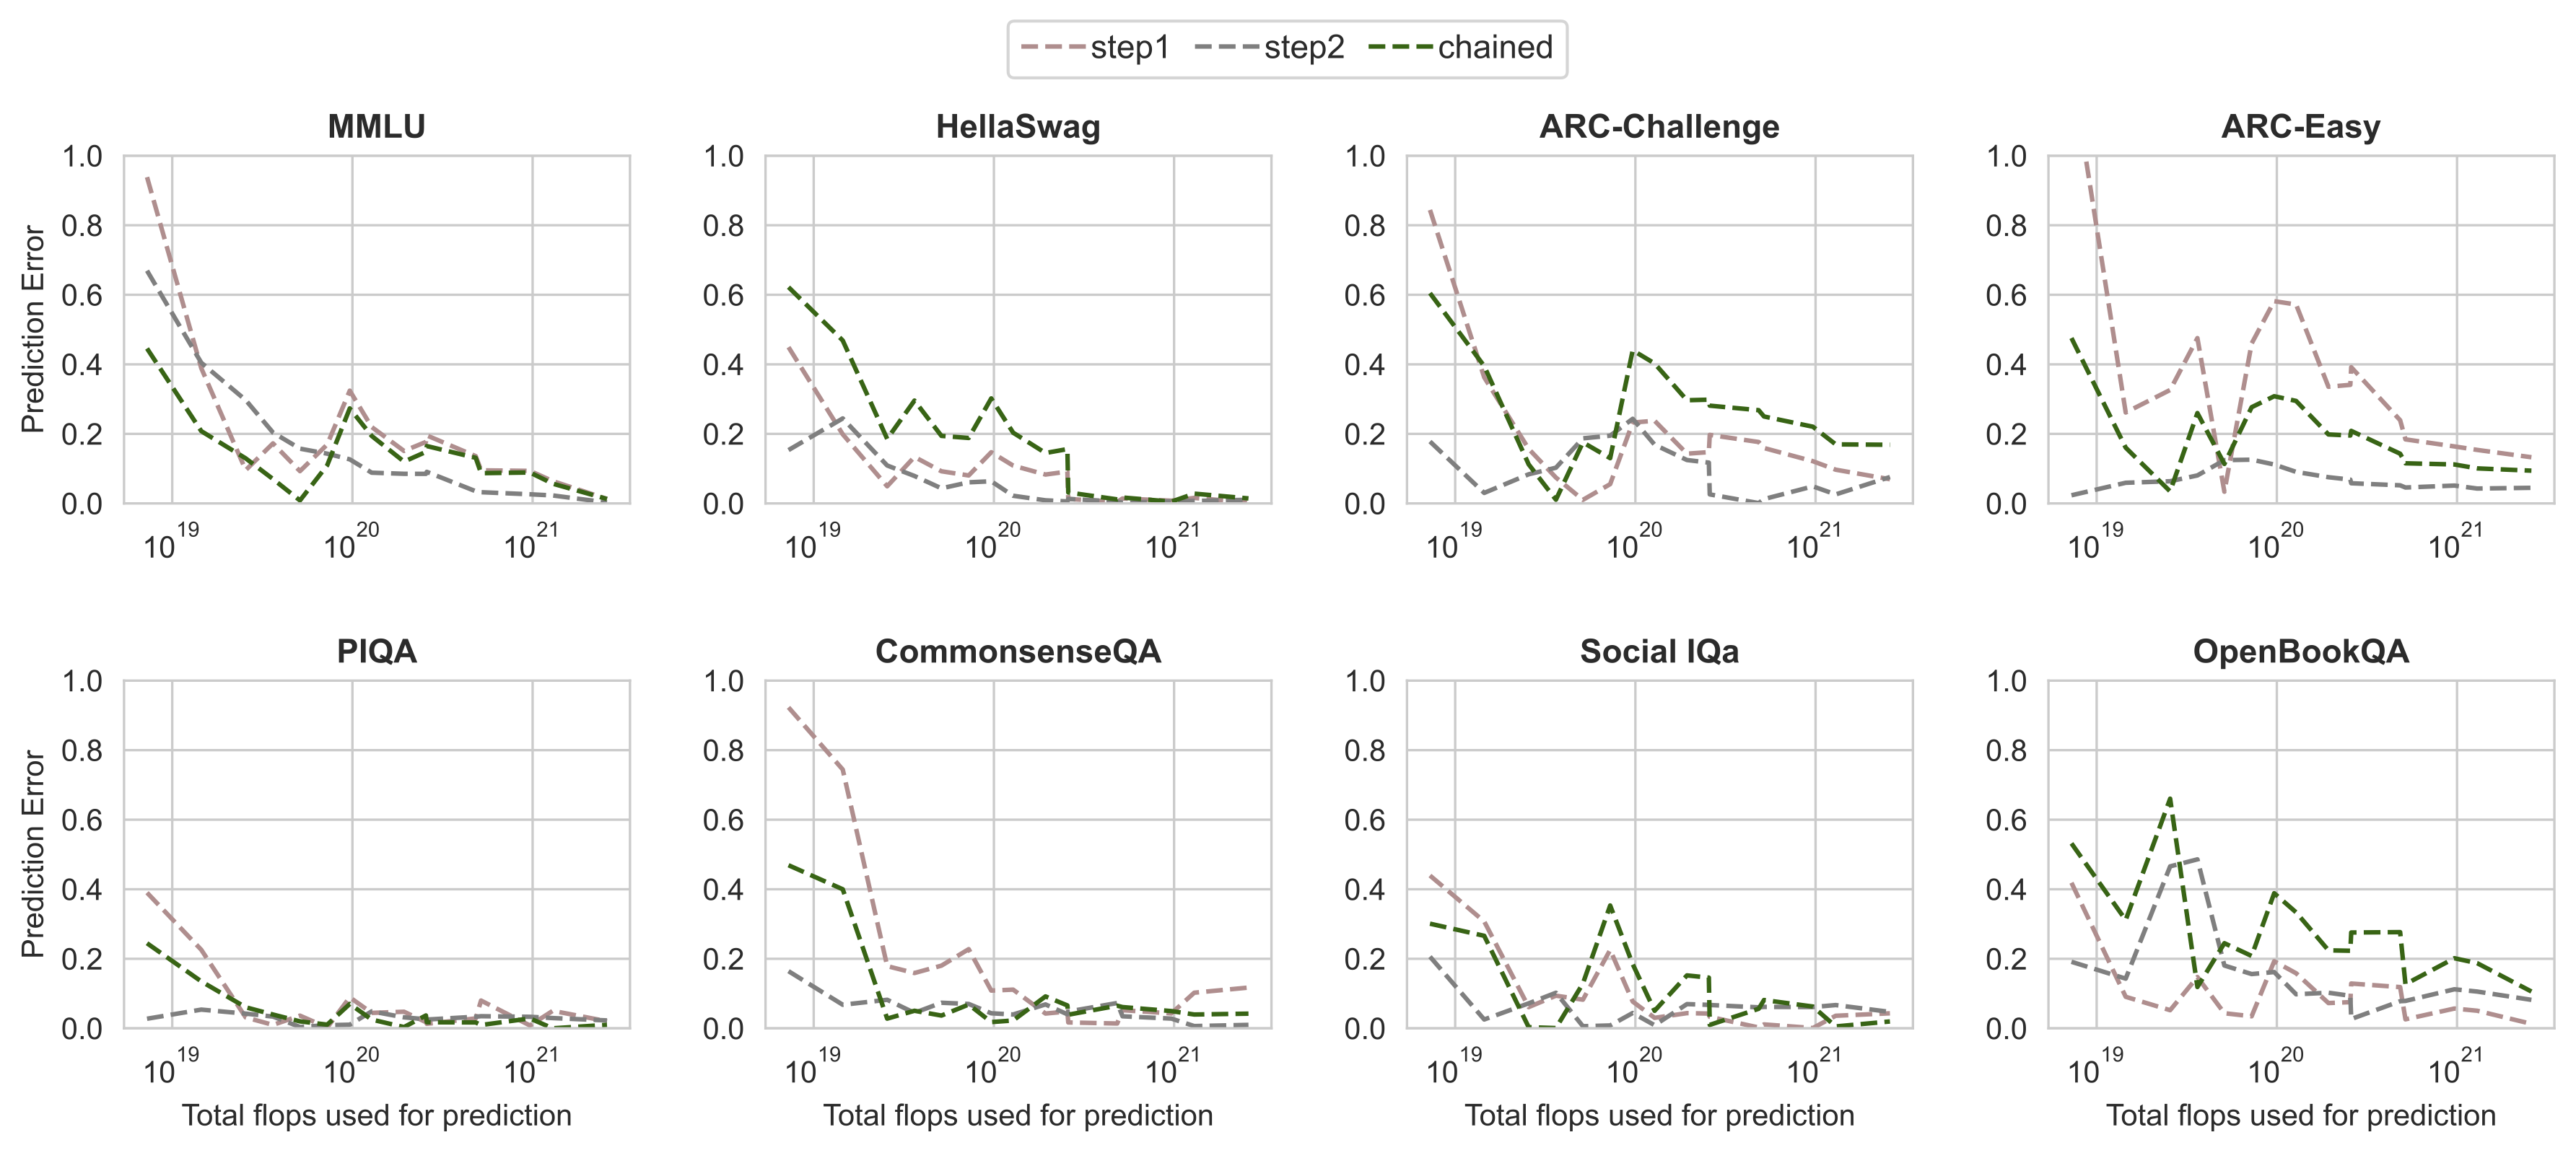
\includegraphics[width=0.8\linewidth]{images/compute_vs_error/vary_flops_error_all.png}
\vspace{-12pt}
\caption{
    Prediction error on the 7B-4T target model as a function of the total compute-FLOPs used in the ladder models for prediction. The left-most point uses only the smallest model (190M-1xC) for prediction. The right-most point uses the full ladder (all 16 models). The prediction error generally reduces as the ladder FLOPs increase. ARC-C, ARC-E, and OBQA display higher variation (which can be attributed to the variation analysis in \S\ref{sec_variance_analysis}), but still have a downward trend.
}
\label{fig:compute_vs_error_flops}
\vspace{-8pt}
\end{figure*}


% \subsection{Compute requirements for predicting each task}
% \label{sec:ablate_compute}

% \akshita{given previous proposed rewrites, this section seems somewhat filler, can move to appendix}

% We consider the impact of the scale of the model ladder on the prediction for the target model. In general, the prediction is harder if the difference of scale between the ladder and the target models is larger. We explore this trade-off using the \textbf{7B-4T} model as the target. 

% In \autoref{fig:compute_vs_error_flops}, we progressively increase the compute-FLOPs used for function fitting. 
%  The prediction error is significantly worse with fewer FLOPs. On MMLU, our full ladder (3.2\% compute of the target model) gets 1.3\% error. Reducing the number of FLOPs to 0.1\% of the target model compute increases the error to $\sim$12\% which is an order of magnitude higher. This is more observable in certain tasks. Interestingly, we see a slight improvement in errors with less compute in ARC-C and ARC-E, potentially due to the variance as seen in \S\ref{sec_variance_analysis}. The impact of each axis of the ladder models (model size $N$ and Chinchilla multiplier $xC$) on the prediction error for each task is discussed in \S\ref{flops_needed}.



% We also consider the impact of each axis of the ladder models (model size $N$ and Chinchilla multiplier $xC$) on the prediction error for each task. 

% \autoref{fig:compute_vs_error_N} shows the prediction errors for each step as we progressively increase the model size included in the ladder (i.e., ladder upto 760M will include 190M, 370M, 760M). We observe a downward trend in the prediction error for most tasks as the ladder size gets closer to the target model. 

% \begin{figure*}[t]
\centering
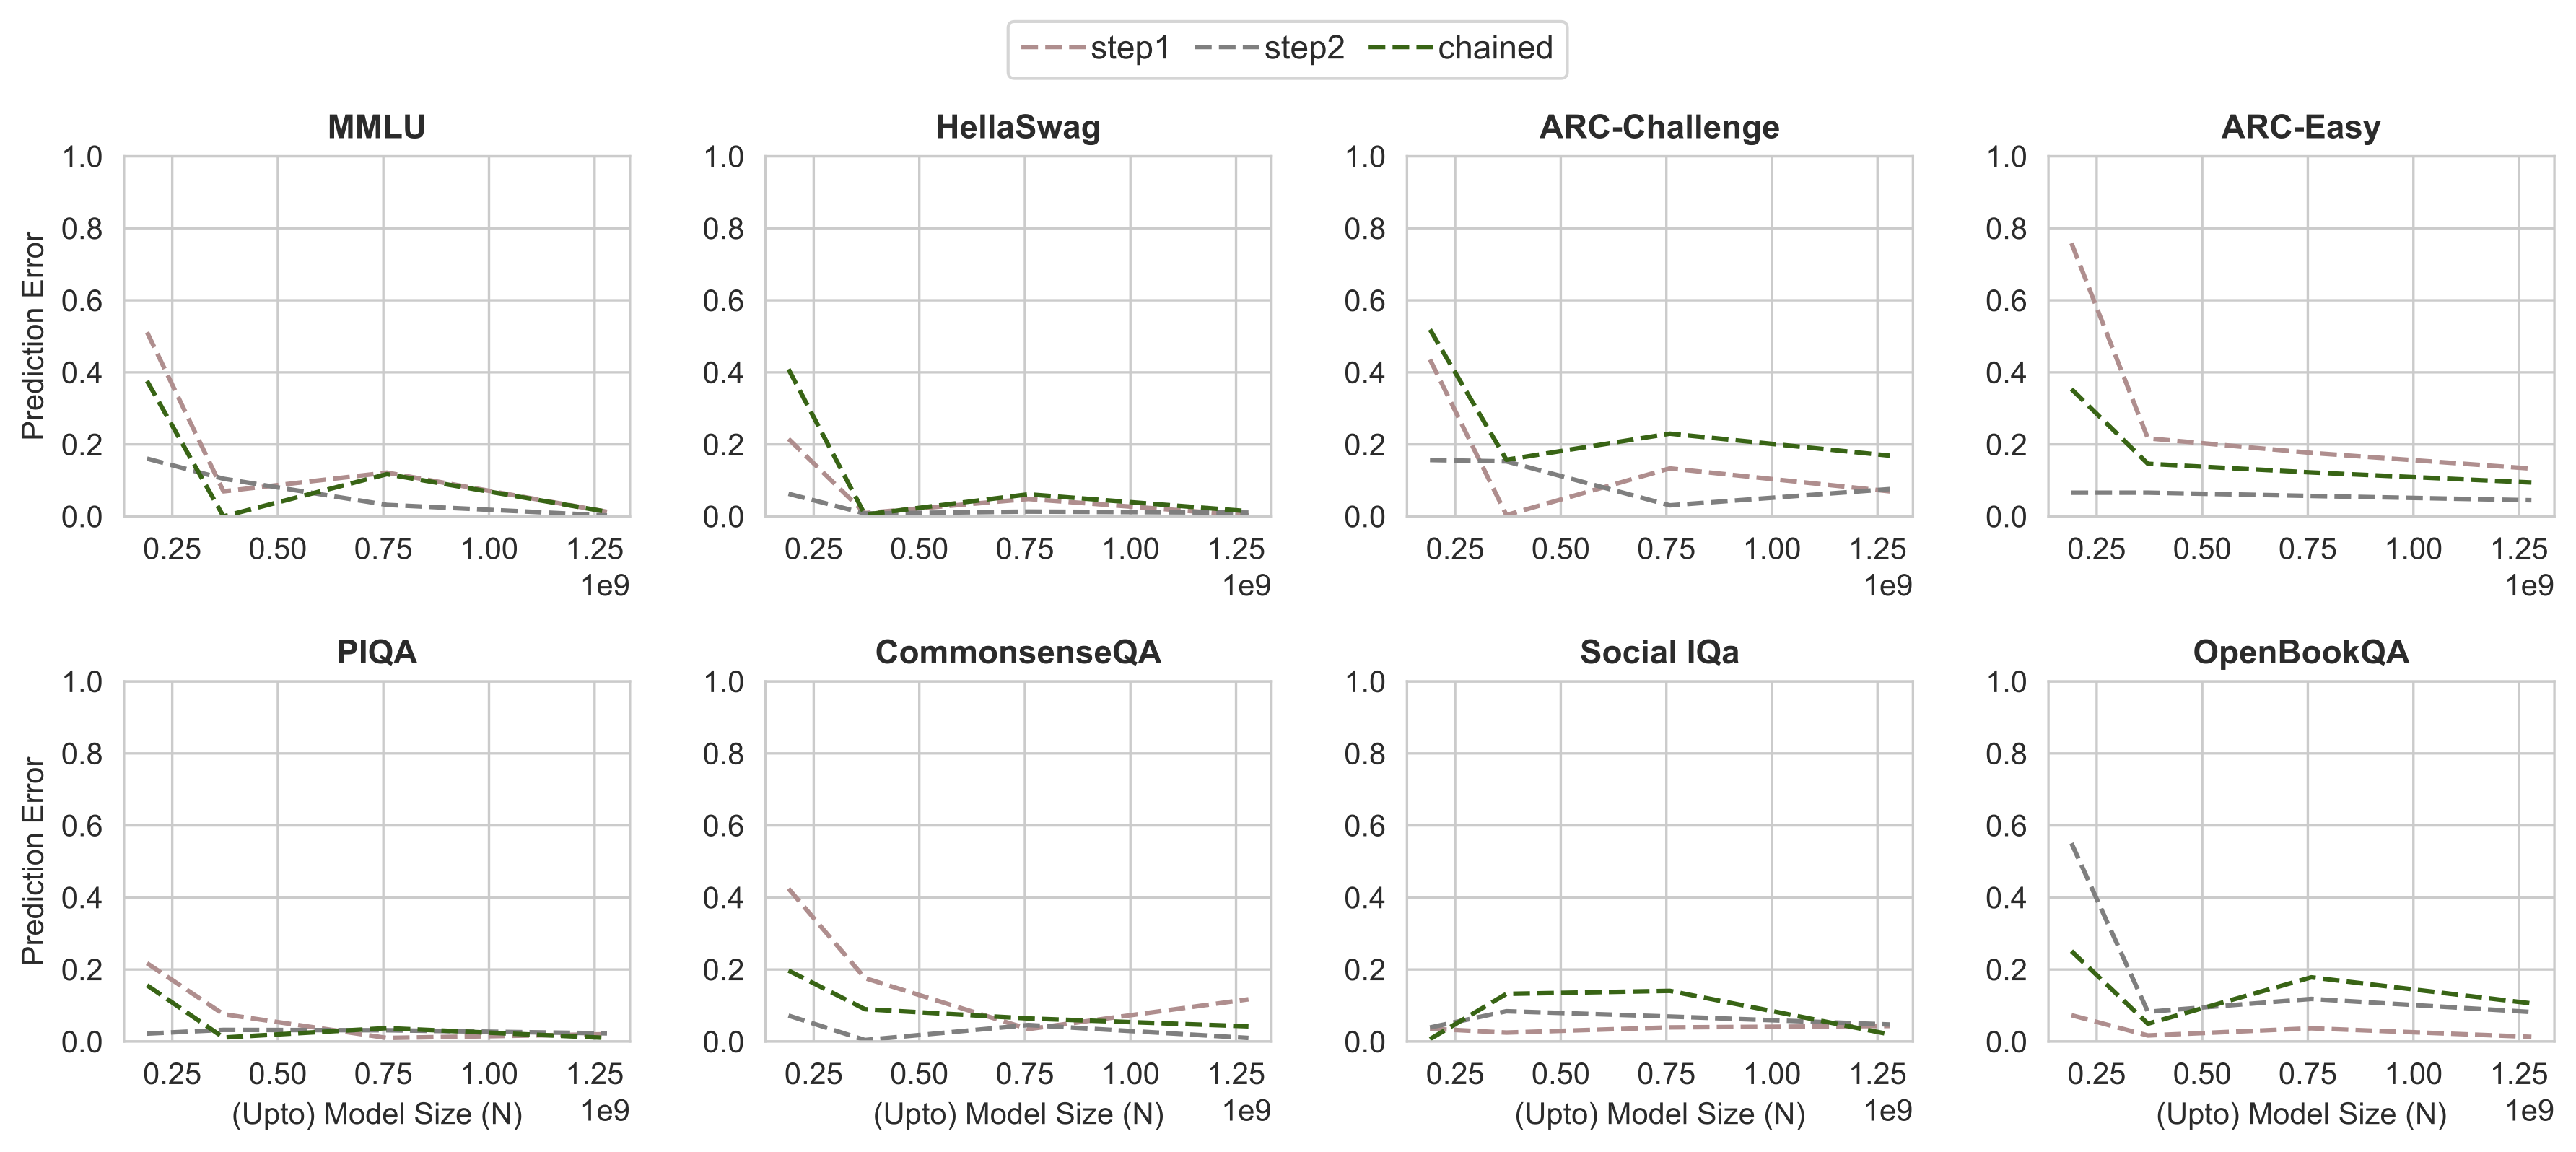
\includegraphics[width=0.90\linewidth]{images/compute_vs_error/vary_N_error_all.png}
\vspace{-12pt}
\caption{
    Prediction error on the 7B-4T target model when including \textbf{up to} model size ($N$) in the ladder for prediction. Eg. $N$ up to 760M will include 190M, 370M, 760M models trained to 1xC, 2xC, 5xC, 10xC. For most tasks, we observe a downward trend in the prediction error as $N$ increases.
}
\label{fig:compute_vs_error_N}
\vspace{-8pt}
\end{figure*}

% \autoref{fig:compute_vs_error_xC} similarly shows the impact of including models with longer training regimes. Interestingly, we do not see a significant reduction in the prediction error as we include the ladder models trained to higher Chinchilla multipliers\footnote{The target model 7B-4T is trained to approximately 28xC.}. There is a slight downward trend (noticeable in MMLU), but this dimension has more flexibility. 

% For users of our approach, and future work, we encourage exploration in reducing the overall cost by considering both these dimensions. Concretely, given a fixed budget for the ladder models, increasing the model size $N$ is more likely to improve the prediction error, compared to training for longer.

% \begin{figure*}[t]
\centering
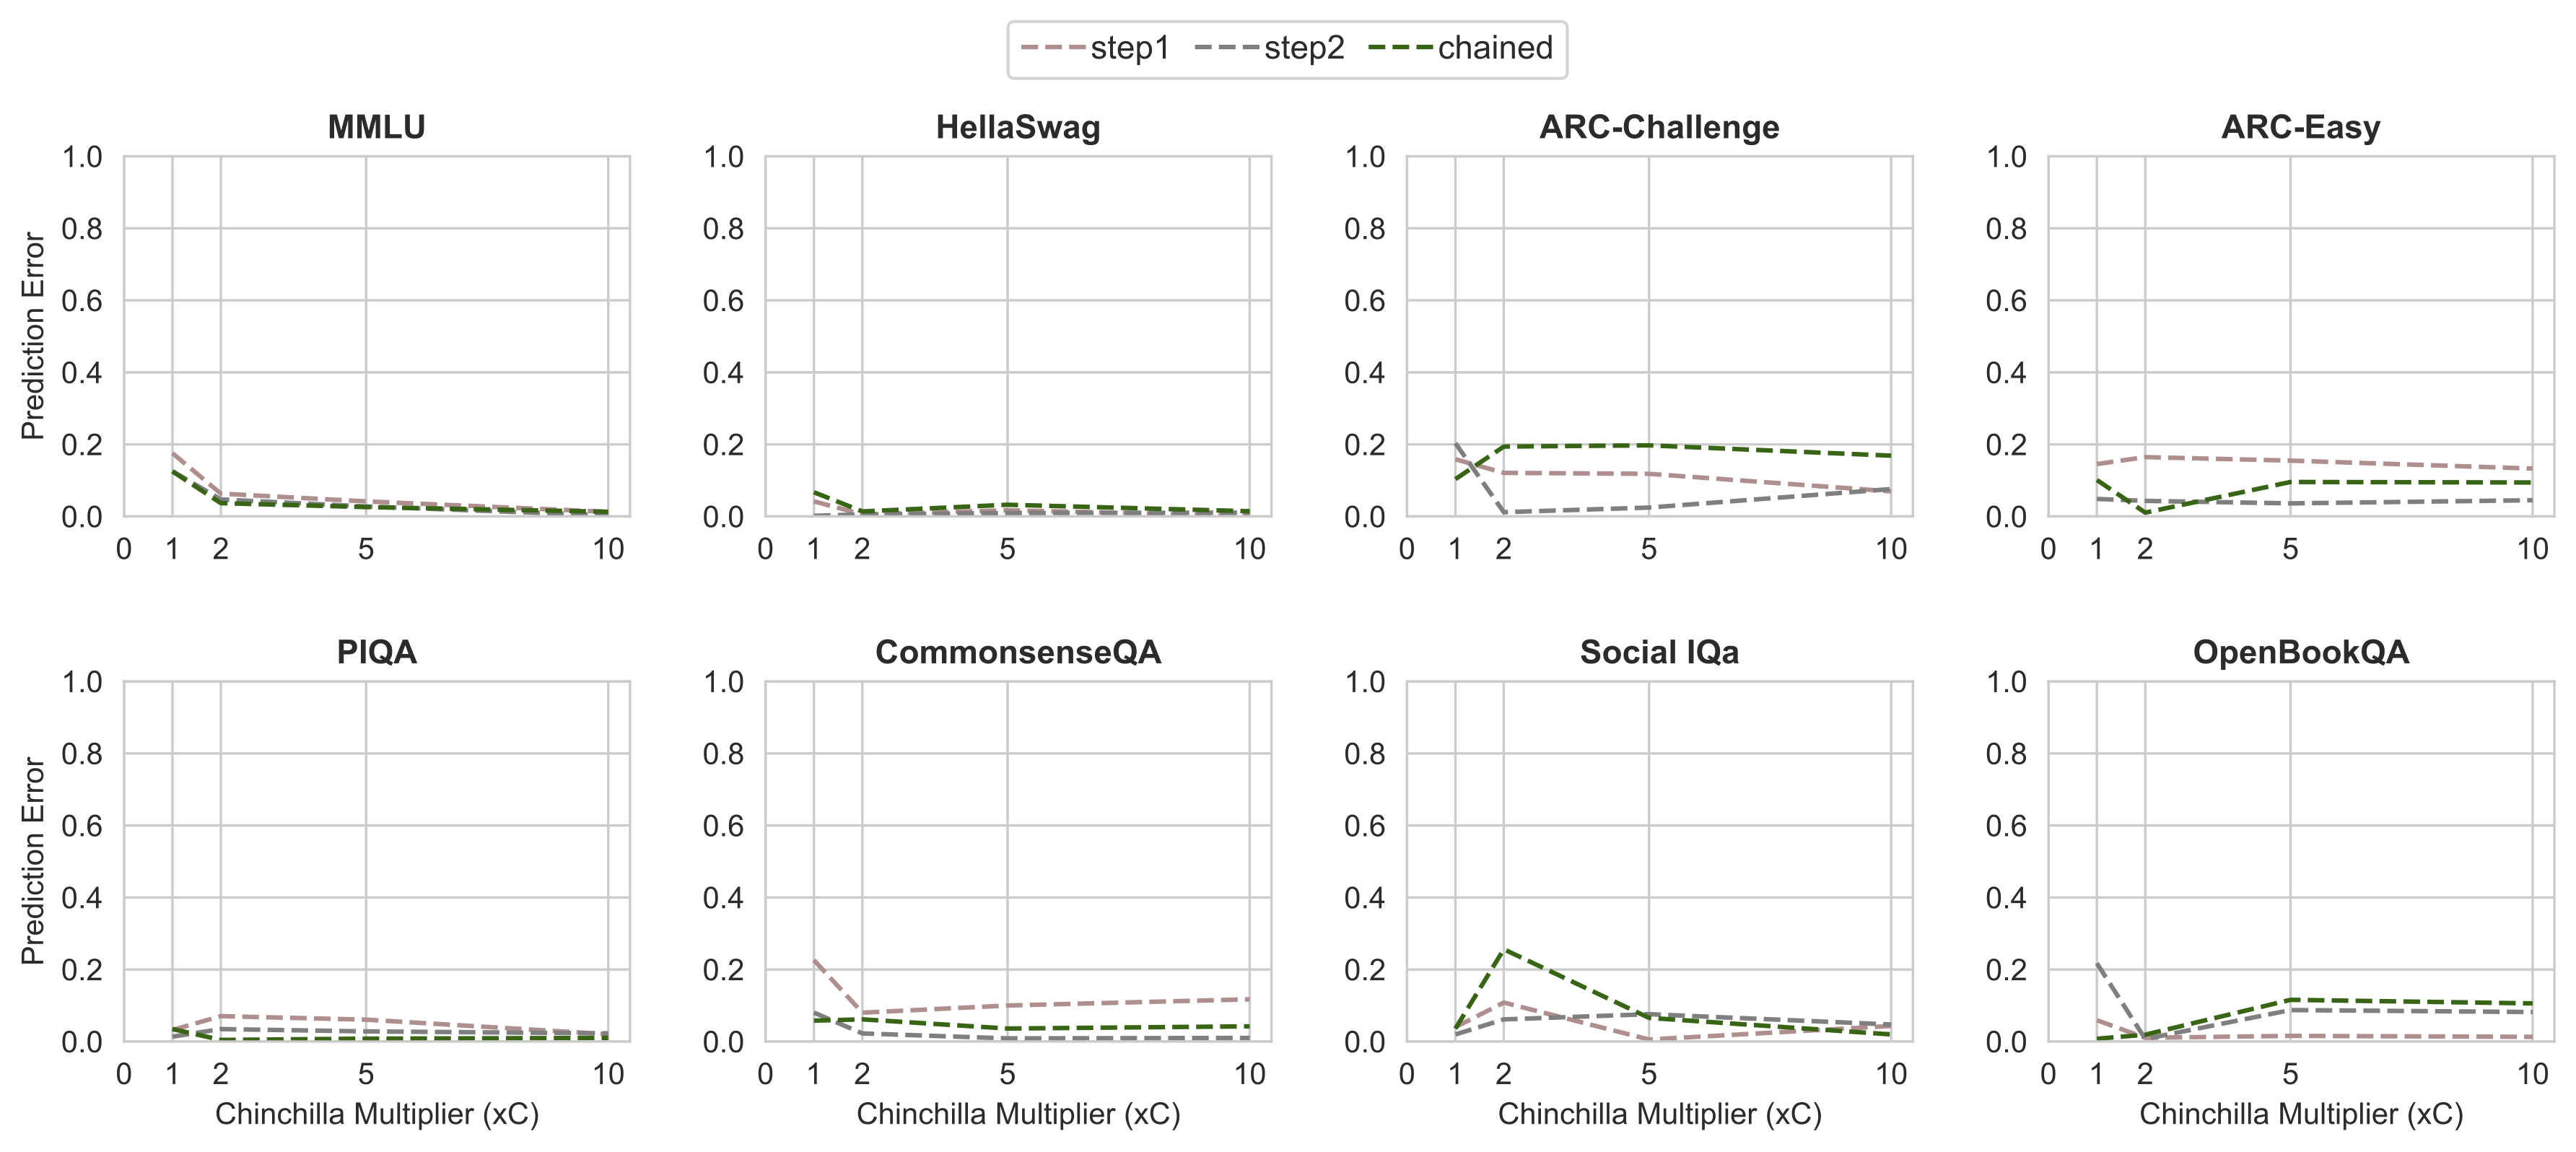
\includegraphics[width=0.90\linewidth]{images/compute_vs_error/vary_xC_error_all.png}
\vspace{-12pt}
\caption{
    Prediction error on the 7B-4T target model when including models trained \textbf{up to} chinchilla multiplier ($xC$). Eg. $xC$ up to 2xC will include 190M, 370M, 760M, 1B models trained to 1xC, 2xC. The downward trend of the prediction error is less significant than with varying $N$. 
}
\label{fig:compute_vs_error_xC}
\vspace{-8pt}
\end{figure*}
